\section{Описание продукций и услуг}

\subsection{Физическое описание услуги}

ООО "Astadeer" предлагает сервис онлайн-персонализации одежды и аксессуаров.  В основе сервиса лежит \textbf{инновационная онлайн-платформа}, доступная через веб-сайт и мобильное приложение.  Платформа представляет собой интуитивно понятный и визуально привлекательный \textbf{конструктор}, где клиенты могут создавать уникальные дизайны на выбранных ими базовых моделях одежды и аксессуаров.

\vspace{0.3cm}

\textbf{Процесс персонализации выглядит следующим образом:}

\begin{enumerate}[label=\arabic*.]
    \item  \textbf{Выбор базового изделия:} Клиент выбирает из каталога доступных товаров: футболки, толстовки, свитшоты, кепки, сумки, чехлы для телефонов и другие аксессуары.  Каждое изделие представлено с качественными \textbf{фотографиями и подробным описанием} материалов, размеров и цветов.
    \item [2. ] \textbf{Переход в онлайн-конструктор:}  Выбрав изделие, клиент переходит в удобный онлайн-конструктор (рисунок \ref{fig:editor}).  Конструктор представляет собой визуальный редактор, где можно \textbf{добавлять изображения, текст, логотипы, использовать готовые графические элементы и менять цвета} элементов дизайна.
    \item [3. ] \textbf{Использование AI-помощника (опционально):}  Клиент может воспользоваться встроенным \textbf{AI-помощником}, который предлагает идеи дизайна, цветовые сочетания, композиции и другие креативные подсказки, облегчая процесс создания уникального стиля.
    \item [4. ] \textbf{Консультация с дизайнером (опционально):}  Для более сложных задач или для получения профессионального совета, клиент может заказать \textbf{консультацию с профессиональным дизайнером} через платформу.
    \item [5. ] \textbf{Предварительный просмотр и заказ:}  В любой момент процесса клиент может увидеть \textbf{предварительный просмотр} созданного дизайна на выбранном изделии.  Удовлетворившись результатом, клиент оформляет заказ, выбирая способ оплаты и доставки.
    \item [6. ] \textbf{Производство и доставка:}  После оформления заказа, персонализированное изделие отправляется в производство.  ООО "Astadeer" гарантирует \textbf{качественное нанесение дизайна} с использованием современных технологий печати и \textbf{экологически чистых материалов}.  Готовое изделие доставляется клиенту выбранным способом (курьером, почтой или самовывозом).
\end{enumerate}

\begin{figure}
    \centering
    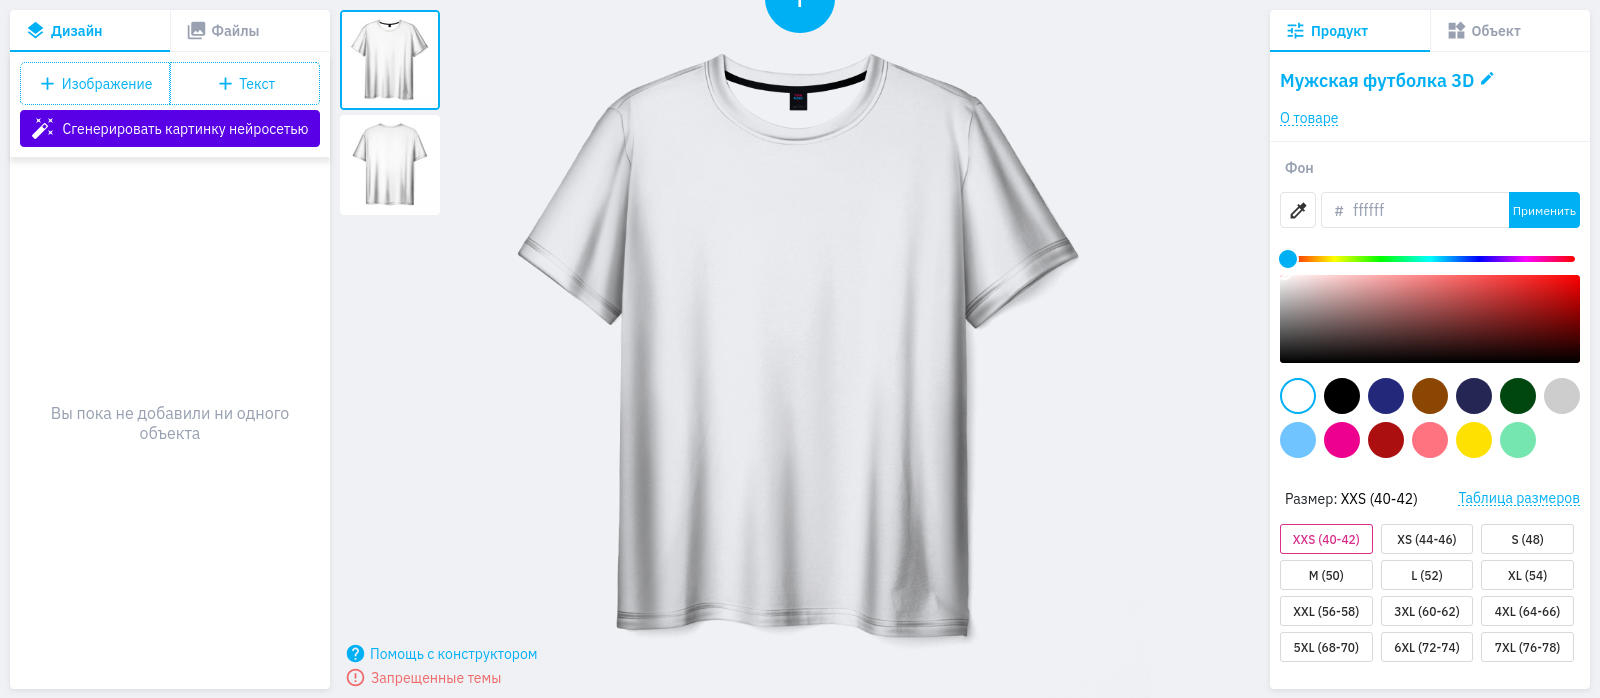
\includegraphics[width=\textwidth]{img/editor.png}
    \caption{Пример вида онлайн-коструктора}
    \label{fig:editor}
\end{figure}

\vspace{0.3cm}

\textbf{Физическим результатом услуги} является готовое персонализированное изделие: футболка с уникальным принтом, толстовка с фотографией, кепка с логотипом и т.д.  Изделия отличаются \textbf{высоким качеством материалов и печати}, а также \textbf{уникальным дизайном}, созданным самим клиентом.

\subsection{Описание возможностей использования}

Сервис ООО "Astadeer" предоставляет широкие возможности для использования персонализированной одежды и аксессуаров в различных ситуациях и для разных целей:

\begin{itemize}
    \item \textbf{Самовыражение и индивидуальный стиль:}  Клиенты могут создавать одежду и аксессуары, которые полностью отражают их личный вкус, интересы и индивидуальность, выделяясь из толпы и подчеркивая свой уникальный стиль.
    \item \textbf{Оригинальные подарки:}  Персонализированные изделия являются отличным вариантом для \textbf{уникальных и запоминающихся подарков} на любые праздники и события.  Подарок, созданный с учетом индивидуальности получателя, всегда ценится особенно высоко.
    \item \textbf{Корпоративная одежда и мерч:}  Сервис идеально подходит для создания \textbf{корпоративной одежды с логотипом компании, мерча для мероприятий, промо-акций и корпоративных подарков}.  Персонализированная продукция способствует повышению узнаваемости бренда и формированию командного духа.
    \item \textbf{Одежда для мероприятий и групп по интересам:}  Можно создавать одежду для \textbf{спортивных команд, фан-клубов, тематических вечеринок, девичников/мальчишников, выпускных и других мероприятий}.  Персонализированная одежда помогает создать единство и подчеркнуть общую идею мероприятия.
    \item \textbf{Продвижение личного бренда и творчества:}  Блогеры, художники, музыканты и другие творческие личности могут использовать сервис для создания \textbf{мерча со своим дизайном и символикой} для продажи своим поклонникам и продвижения своего личного бренда.
    \item \textbf{Создание уникальных коллекций одежды:}  Начинающие дизайнеры и энтузиасты моды могут использовать платформу для \textbf{экспериментов с дизайном и создания небольших авторских коллекций} персонализированной одежды для продажи или личного использования.
\end{itemize}

\subsection{Привлекательные стороны продукта или услуги}

Сервис онлайн-персонализации ООО "Astadeer" обладает рядом привлекательных сторон для клиентов:

\begin{itemize}
    \item \textbf{Уникальность и персонализация:}  Возможность создать абсолютно уникальный продукт, отражающий индивидуальность клиента, что отвечает растущему тренду на персонализацию и самовыражение.
    \item \textbf{Удобство и простота использования:}  Интуитивно понятная онлайн-платформа делает процесс дизайна легким и увлекательным даже для пользователей без специальных навыков.
    \item \textbf{Инновационный AI-помощник:}  Встроенный AI-помощник предлагает креативные идеи и упрощает процесс дизайна, делая его доступным и вдохновляющим.
    \item \textbf{Экологичность:}  Использование экологически чистых материалов и технологий печати отвечает современным требованиям к устойчивому производству и привлекает экологически осознанных клиентов.
    \item \textbf{Качество:}  Гарантия высокого качества материалов и печати обеспечивает долговечность и привлекательный внешний вид персонализированной продукции.
    \item \textbf{Возможность консультаций с дизайнерами:}  Предоставление профессиональной поддержки для клиентов, которым требуется помощь в создании сложных дизайнов, повышает ценность сервиса.
    \item \textbf{Широкий ассортимент базовых моделей:}  Разнообразие выбора одежды и аксессуаров для персонализации позволяет удовлетворить различные вкусы и потребности.
    \item \textbf{Быстрое изготовление и удобная доставка:}  Оперативность выполнения заказов и различные варианты доставки обеспечивают комфорт и удовлетворенность клиентов.
    \item \textbf{Конкурентоспособные цены:}  Сервис предлагает хорошее соотношение цены и качества, делая персонализированную одежду доступной для широкого круга потребителей.
\end{itemize}

\subsection{Новизна характеристик товара}

Новизна сервиса ООО "Astadeer" заключается в следующем сочетании характеристик:

\begin{itemize}
    \item \textbf{Интеграция AI-помощника в онлайн-платформу персонализации:}  Внедрение интеллектуального AI-помощника для дизайна является инновационным решением на рынке персонализированной одежды и аксессуаров.  AI-помощник не только упрощает процесс создания дизайна, но и предлагает персонализированные рекомендации, расширяя творческие возможности клиентов и отличая платформу от конкурентов.
    \item \textbf{Сочетание персонализации и экологичности:}  ООО "Astadeer" предлагает комплексный сервис, сочетающий возможность создания уникального продукта и использование экологически чистых материалов.  Такое сочетание является важным конкурентным преимуществом на современном рынке.
    \item \textbf{Возможность консультаций профессиональных дизайнеров:}  Для клиентов, которым требуется профессиональная помощь и экспертное мнение, ООО "Astadeer" предоставляет возможность получить консультации от квалифицированных дизайнеров. Это повышает ценность сервиса и привлекает клиентов, стремящихся к безупречному результату.
\end{itemize}

\subsection{Степень готовности продукта или услуги к выходу на рынок}

На текущий момент, сервис ООО "Astadeer" находится на стадии \textbf{MVP (Minimum Viable Product) – минимально жизнеспособного продукта}.

\vspace{0.3cm}

\textbf{Степень готовности к выходу на рынок можно охарактеризовать следующим образом:}

\begin{itemize}
    \item \textbf{Разработана и протестирована базовая функциональность онлайн-платформы (веб-сайт и мобильное приложение):}  Основные функции конструктора, каталога товаров, оформления заказа, оплаты и доставки разработаны и проходят стадию внутреннего тестирования.
    \item \textbf{Сформирован каталог базовых моделей одежды и аксессуаров для персонализации (более 50 позиций):}  Ассортимент MVP включает в себя наиболее востребованные категории товаров для персонализации.
    \item \textbf{Интегрирован AI-помощник для дизайна (базовая версия):}  Функциональность AI-помощника реализована в базовом варианте и будет расширяться по мере развития платформы.
    \item \textbf{Проведены предварительные тесты удобства использования платформы с фокус-группой потенциальных пользователей:}  Получена положительная обратная связь, выявлены области для улучшения интерфейса и функциональности.
    \item \textbf{Заключены предварительные договоренности с поставщиками экологически чистых материалов и производителями печати:}  Обеспечена производственная база для запуска MVP.
    \item \textbf{Разработана базовая маркетинговая стратегия и план продвижения MVP:}  Подготовлены материалы для запуска рекламных кампаний и привлечения первых пользователей.
\end{itemize}

\vspace{0.3cm}

\textbf{Следующим шагом является запуск MVP онлайн-платформы для ограниченного круга пользователей (бета-тестирование), сбор обратной связи и доработка платформы перед полноценным выходом на рынок.}  Опытная партия персонализированной продукции будет произведена в рамках бета-тестирования для отладки производственных процессов и проверки качества.

\subsection{Список экспертов или потребителей, которые знакомы с товарами или услугами и могут дать положительные отзывы}

На стадии MVP и подготовки к запуску, ООО "Astadeer" активно взаимодействует с экспертами и потенциальными потребителями, в частности, фокусируясь на студенческой аудитории крупных белорусских вузов, таких как БГУИР и БГУ, как на одном из ключевых сегментов целевого рынка.

\vspace{0.3cm}

\textbf{Список экспертов и потребителей, знакомых с сервисом и потенциально готовых дать положительные отзывы (на стадии формирования):}

\begin{itemize}
    \item \textbf{Потребители – студенты БГУИР и БГУ (участники фокус-группы и потенциальные клиенты):}
        \begin{itemize}
            \item \textbf{Фокус-группа студентов БГУИР и БГУ (20 человек):}  Фокус-группа была сформирована из студентов различных факультетов БГУИР и БГУ, представляющих активную часть студенческого сообщества.  Критерии отбора включали: \textbf{активное использование социальных сетей, опыт онлайн-покупок, интерес к моде и индивидуальному стилю, участие в студенческой жизни}.  Студенты протестировали бета-версию платформы, оценивая ее удобство, функциональность и привлекательность ассортимента с точки зрения их потребностей. \textbf{В отзывах студентов БГУИР и БГУ особо отмечались:}  \textbf{удобство создания дизайна для университетского мерча (для факультетов, групп, студенческих организаций), возможность заказать уникальные подарки для одногруппников и друзей, а также желание использовать сервис для самовыражения и создания одежды в своем индивидуальном стиле.}
            \item \textbf{Студенческие организации и инициативные группы БГУИР и БГУ:}  Ведутся \textbf{предварительные переговоры с представителями студенческих советов и активов факультетов БГУИР и БГУ}  о возможности использования платформы "Astadeer" для создания \textbf{персонализированного мерча для студенческих мероприятий, спортивных команд, научных кружков и других студенческих объединений}.  Несколько студенческих организаций БГУИР и БГУ выразили заинтересованность в проведении тестовых заказов для своих нужд после запуска платформы.
        \end{itemize}
\end{itemize}

\vspace{0.3cm}

**Важно отметить, что взаимодействие с экспертами и студентами БГУИР и БГУ продолжается на этапе MVP.  По мере развития проекта и получения первых заказов от студентов и студенческих организаций, список положительных отзывов и примеров успешного использования сервиса будет расширяться и уточняться.**